\section{Experimental Evaluation}
\label{sec:experiments}

We evaluate predictive performance, component allocation, communication cost, and representation fidelity. A matched CIFAR-100 study examines the MiSFP mechanisms, while broader classification and segmentation benchmarks provide context across tasks.

\subsection{Experimental Setup}

\noindent\textbf{Datasets and partitions.} Classification experiments cover CIFAR-10, CIFAR-100, HAM10000, and ImageNet-1K. ISIC-2018 segmentation uses the spatial-feature formulation in Section~\ref{subsec:segmentation}. The matched CIFAR-100 study considers IID partitions and Dirichlet partitions with $\alpha\in\{0.7,0.1\}$; smaller $\alpha$ produces greater variation in client class proportions. The broader CIFAR-100 benchmark additionally includes Dir($\alpha=0.3$).

\noindent\textbf{Training configuration.} The matched study uses 200 clients assigned to five edge servers, with 10\% participation per round. Training lasts 200 rounds using Adam, a learning rate of $10^{-4}$, and a local batch size of 16. The client encoder comprises ResNet-18 through layer~2 followed by global average pooling, producing $d_{ce}=128$ features. The edge maps these features to $d_{ec}=256$. Synchronization uses $t_1=5$ and $t_2=10$, following \cref{sec:method}.
We reserve 10\% of the standard CIFAR-100 training set for validation and retain the standard test set for evaluation. This dataset-level validation split is separate from the local split used for adaptive component selection. The focused study comprises 31 configurations evaluated with seeds $\{1,2,3\}$, giving 93 runs. \Cref{tab:setup} summarizes the configuration.

\begin{table*}[t]
\caption{Configuration of the matched CIFAR-100 study.}
\label{tab:setup}
\centering
\footnotesize
\begin{tabularx}{\textwidth}{@{}lXlX@{}}
\toprule
Setting & Value & Setting & Value\\
\midrule
Dataset/task & CIFAR-100 classification (100 classes) & Topology & 200 clients, five edges; 10\% participation\\
Data split & Standard train/test; 10\% of training data reserved for validation & Partitions & IID, Dir($\alpha=0.7$), Dir($\alpha=0.1$)\\
Model/split & ResNet-18; 128/256-dimensional boundaries & Training & Adam, learning rate $10^{-4}$, batch size 16\\
Evaluation & Round 200; seeds $\{1,2,3\}$ & Runs & 31 configurations; 93 runs\\
Metrics & Accuracy, macro-F1, fidelity, communication & Synchronization & $t_1=5$, $t_2=10$\\
\bottomrule
\end{tabularx}
\end{table*}

\noindent\textbf{Baselines and comparison protocols.} H-SFP is the matched baseline in the five-edge study. MiSFP-K1 uses single-component moment pooling; Edge retains components across sources; K2 and K4 additionally permit fixed local mixtures; and Adaptive selects local component counts using held-out likelihood. \cref{tab:variants} distinguishes requested local counts from hierarchical retention limits.
The broader benchmarks include federated, hierarchical, split-learning, and feature-transfer methods. These tables provide descriptive benchmark context across the reported settings.

\noindent\textbf{Metrics and reporting.} Classification uses top-1 accuracy and macro-F1; segmentation uses foreground intersection over union (IoU) and Dice. Entries report mean $\pm$ standard deviation (SD). Differences between percentage metrics are expressed in percentage points and computed from the reported means. SDs describe run-to-run variability; they are not confidence intervals or significance tests.

Representation fidelity is evaluated on held-out real features using negative log likelihood per dimension (NLL), sliced Wasserstein distance (SWD), and maximum mean discrepancy (MMD). Lower values indicate better agreement under the corresponding criterion. Each mixture--collapse comparison uses the same split boundary and feature definition. Distributional comparisons are made in raw feature coordinates, separately from the normalization used by the receiving predictor. Encoder compatibility is examined through the ratio of between-source to total feature dispersion.

Communication accounts for complete serialized prototype packets at both boundaries and model-synchronization traffic. Packet headers are included. Communication and memory are reported in MiB, where $1\,\mathrm{MiB}=2^{20}$ bytes; runtime is reported in seconds unless stated otherwise. Focused resource measurements were collected on a shared RTX 6000 Ada GPU and are interpreted within that execution setting.

\subsection{Predictive Performance}
\label{sec:results}

\noindent\textbf{Matched CIFAR-100 comparison.} \Cref{tab:main} reports the controlled comparison across three partitions. MiSFP-K4 improves on the H-SFP accuracy mean by 4.91, 4.40, and 3.97\% under IID and $\alpha\in\{0.7;0.1\}$, respectively. K2 has the highest IID mean, while K4 has the highest means under two heterogeneous setups. Under $\alpha=0.1$, K4 reaches $7.88\pm0.45\%$ macro-F1 compared with $4.45\pm0.29\%$ for H-SFP.

\begin{table*}[t]
\caption{Matched CIFAR-100 results after 200 rounds: mean $\pm$ SD over three seeds. K1 uses single-component pooling; Edge retains components across sources; K2, K4, and Adaptive additionally permit within-client mixtures. F1 denotes macro-F1.}
\label{tab:main}
\centering
\footnotesize
\setlength{\tabcolsep}{3pt}
\begin{tabular*}{\textwidth}{@{\extracolsep{\fill}}lcccccc@{}}
\toprule
& \multicolumn{2}{c}{IID} & \multicolumn{2}{c}{Dir($\alpha=0.7$)} & \multicolumn{2}{c}{Dir($\alpha=0.1$)}\\
\cmidrule(lr){2-3}\cmidrule(lr){4-5}\cmidrule(lr){6-7}
Method & Acc. (\%) & F1 (\%) & Acc. (\%) & F1 (\%) & Acc. (\%) & F1 (\%)\\
\midrule
H-SFP & $55.10\pm0.38$ & $53.51\pm0.42$ & $10.48\pm0.28$ & $8.99\pm0.38$ & $5.49\pm0.36$ & $4.45\pm0.29$\\
MiSFP-K1 & $54.93\pm0.06$ & $53.12\pm0.12$ & $9.70\pm0.10$ & $7.82\pm0.09$ & $5.12\pm0.11$ & $3.54\pm0.37$\\
MiSFP-Edge & $59.87\pm0.23$ & $57.57\pm0.17$ & $13.80\pm0.45$ & $11.53\pm0.35$ & $6.82\pm0.06$ & $4.85\pm0.35$\\
MiSFP-K2 & $60.05\pm0.35$ & $57.82\pm0.28$ & $14.81\pm0.59$ & $12.67\pm0.57$ & $8.75\pm0.16$ & $7.06\pm0.29$\\
MiSFP-K4 & $60.01\pm0.36$ & $57.76\pm0.29$ & $14.88\pm0.56$ & $12.71\pm0.56$ & $9.46\pm0.31$ & $7.88\pm0.45$\\
MiSFP-Adaptive & $59.87\pm0.23$ & $57.57\pm0.17$ & $13.82\pm0.35$ & $11.58\pm0.29$ & $7.50\pm0.14$ & $5.67\pm0.28$\\
\bottomrule
\end{tabular*}
\end{table*}

The severe-partition accuracy remains low even for K4. Its improvement demonstrates a comparative benefit within the tested configuration, while the $9.46\%$ endpoint limits claims about practical deployment under extreme heterogeneity. Component retention addresses one source of approximation in the hierarchical training pipeline; these results do not establish that it resolves the broader optimization difficulties of this setting.

\noindent\textbf{Classification across datasets.} \Cref{tab:classification200} reports IID classification accuracy after 200 rounds. MiSFP-K4 has the highest listed mean on CIFAR-10, CIFAR-100, HAM10000, and ImageNet-1K. Fig.~\ref{fig:empirical}(a) summarizes its comparison with H-SFP. The reference baseline statistics retain their published protocol, so these rankings provide broader context alongside the matched results above.

\begin{table*}[t]
\caption{IID classification accuracy (\%) after 200 rounds. Entries report mean $\pm$ SD. Baseline rows are reproduced from~\cite{tran2026h}; HSFL (A) and H-SFP (A) retain the reference configuration labels.}
\label{tab:classification200}
\centering
\begin{tabular*}{\textwidth}{@{\extracolsep{\fill}}lcccc@{}}
\toprule
Method & CIFAR-10 & CIFAR-100 & HAM10000 & ImageNet-1K\\
\midrule
FedAvg & $57.25\pm1.24$ & $48.85\pm1.40$ & $68.28\pm1.45$ & $23.10\pm1.40$\\
FedProx & $58.25\pm1.20$ & $52.75\pm1.25$ & $71.15\pm1.30$ & $24.10\pm1.30$\\
FedNova & $23.50\pm1.15$ & $50.24\pm1.35$ & $69.60\pm1.35$ & $23.80\pm1.30$\\
FedProto & $55.10\pm1.05$ & $46.50\pm1.15$ & $67.20\pm1.25$ & $25.20\pm1.20$\\
HierFL & $62.50\pm1.30$ & $30.15\pm1.45$ & $69.50\pm1.25$ & $24.50\pm1.20$\\
SplitFed & $61.85\pm1.25$ & $35.00\pm1.30$ & $65.78\pm1.35$ & $25.50\pm1.10$\\
HeteroSFL & $63.45\pm1.10$ & $41.50\pm1.25$ & $67.10\pm1.20$ & $26.30\pm0.80$\\
FedGen & $59.80\pm1.10$ & $51.20\pm1.25$ & $72.50\pm1.15$ & $26.80\pm1.00$\\
FedDF & $61.50\pm1.15$ & $53.10\pm1.20$ & $73.10\pm1.20$ & $25.90\pm1.10$\\
HSFL (A) & $51.35\pm1.10$ & $35.47\pm1.35$ & $68.82\pm1.25$ & $24.60\pm0.90$\\
H-SFP (A) & $67.44\pm0.85$ & $55.10\pm0.95$ & $80.86\pm0.75$ & $27.90\pm0.30$\\
\midrule
\textbf{MiSFP-K4} & $\mathbf{72.35\pm1.00}$ & $\mathbf{60.01\pm0.36}$ & $\mathbf{85.77\pm0.91}$ & $\mathbf{32.81\pm0.60}$\\
\bottomrule
\end{tabular*}
\end{table*}

\noindent\textbf{Broader CIFAR-100 comparison.} In \cref{tab:reference}, MiSFP-K4 reaches $11.27\pm0.39\%$ under Dir($\alpha=0.3$) and $14.88\pm0.56\%$ under Dir($\alpha=0.7$), alongside H-SFP reference results of $7.15\pm0.65\%$ and $10.48\pm0.85\%$, respectively. Among the remaining reference methods, FedDF has the highest IID mean and FedGen has the highest means under both heterogeneous partitions.

\begin{table}[t]
\caption{CIFAR-100 top-1 accuracy (\%) after 200 rounds. Entries report mean $\pm$ SD in 5 seeds.}
\label{tab:reference}
\centering
\footnotesize
\setlength{\tabcolsep}{2.5pt}
\begin{tabular*}{\columnwidth}{@{\extracolsep{\fill}}lccc@{}}
\toprule
Method & IID & Dir($\alpha=0.3$) & Dir($\alpha=0.7$)\\
\midrule
FedAvg & $48.85\pm1.40$ & $2.10\pm0.85$ & $5.40\pm1.15$\\
FedSGD & $10.75\pm0.90$ & $1.80\pm0.40$ & $4.35\pm0.65$\\
FedNova & $50.24\pm1.35$ & $3.15\pm0.75$ & $6.80\pm0.95$\\
FedProx & $52.75\pm1.25$ & $4.05\pm0.85$ & $7.20\pm1.10$\\
FedProto & $46.50\pm1.15$ & $6.50\pm0.95$ & $8.80\pm1.05$\\
HierFL & $30.15\pm1.45$ & $1.95\pm0.60$ & $4.78\pm0.85$\\
SplitFed & $35.00\pm1.30$ & $4.15\pm0.80$ & $7.05\pm1.00$\\
HeteroSFL & $41.50\pm1.25$ & $5.45\pm0.70$ & $8.20\pm0.95$\\
FedGen & $51.20\pm1.25$ & $6.70\pm0.85$ & $9.15\pm1.10$\\
FedDF & $53.10\pm1.20$ & $4.50\pm0.70$ & $7.80\pm1.05$\\
HSFL (A) & $35.47\pm1.35$ & $5.10\pm0.80$ & $8.25\pm1.15$\\
H-SFP (A) & $55.10\pm0.95$ & $7.15\pm0.65$ & $10.48\pm0.85$\\
\midrule
\textbf{MiSFP-K4} & $60.01\pm0.36$ & $11.27\pm0.39$ & $14.88\pm0.56$\\
\bottomrule
\end{tabular*}
\end{table}

\noindent\textbf{Segmentation.} On ISIC-2018, MiSFP-K4 achieves $73.21\pm0.72\%$ IoU and $84.41\pm0.66\%$ Dice, compared with H-SFP reference values of $68.30\pm0.50\%$ and $79.50\pm0.40\%$ (\cref{tab:segmentation200}). Fig.~\ref{fig:empirical}(b) presents these foreground-overlap means. The task extends the statistical interface to labeled spatial embeddings. MiSFP runtime is unavailable for this benchmark, so the table does not support a runtime comparison with MiSFP.

\begin{table}[t]
\caption{ISIC-2018 segmentation after 200 rounds.}
\label{tab:segmentation200}
\centering
\footnotesize
\setlength{\tabcolsep}{2.5pt}
\begin{tabular*}{\columnwidth}{@{\extracolsep{\fill}}lccc@{}}
\toprule
Method & IoU (\%) $\uparrow$ & Dice (\%) $\uparrow$ & Time (h) $\downarrow$\\
\midrule
FedAvg & $48.70\pm1.20$ & $64.20\pm1.50$ & $28.5\pm0.8$\\
HierFL & $51.20\pm1.10$ & $66.30\pm1.30$ & $24.3\pm0.7$\\
SplitFed & $53.80\pm0.90$ & $68.10\pm1.10$ & $72.4\pm1.6$\\
HeteroSFL & $56.40\pm0.70$ & $70.50\pm0.80$ & $45.8\pm1.2$\\
HSFL (A) & $62.10\pm0.80$ & $74.80\pm0.90$ & $14.5\pm0.5$\\
H-SFP (A) & $68.30\pm0.50$ & $79.50\pm0.40$ & $6.8\pm0.2$\\
\midrule
\textbf{MiSFP-K4} & $\mathbf{73.21\pm0.72}$ & $\mathbf{84.41\pm0.66}$ & n/r\\
\bottomrule
\end{tabular*}
\end{table}

\begin{figure}[t]
\centering
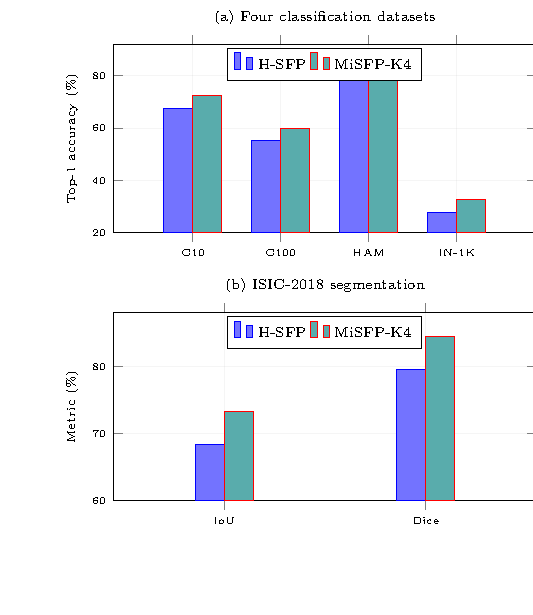
\includegraphics[width=\columnwidth]{figures/empirical_results.pdf}
\caption{Performance after 200 rounds: (a) IID top-1 accuracy on four classification datasets and (b) foreground IoU and Dice on ISIC-2018. Bars show means; SDs are reported in \cref{tab:classification200,tab:segmentation200}. Reference baseline protocols are distinguished from the matched study in the experimental setup.}
\label{fig:empirical}
\end{figure}

\subsection{Component Retention and Sensitivity}

\noindent\textbf{Across-source retention.} MiSFP-K1 has lower reported accuracy means than H-SFP in all three matched partitions (\cref{tab:main}). Retaining source components in MiSFP-Edge raises accuracy relative to K1 throughout: under IID, the mean increases from $54.93\%$ to $59.87\%$, while under Dir($\alpha=0.1$) it increases from $5.12\pm0.11\%$ to $6.82\pm0.06\%$. The results support retaining distinct source components before synthesis within the tested pipeline.

\noindent\textbf{Within-client components.} K2 and K4 provide additional gains over Edge under heterogeneous partitions. Under Dir($\alpha=0.1$), they reach $8.75\pm0.16\%$ and $9.46\pm0.31\%$, respectively, corresponding to gains of 1.93 and 2.64 points over Edge and 3.26 and 3.97 points over H-SFP. Under IID, their means remain close to Edge, indicating that across-source retention accounts for most of the observed improvement in that setting (Fig.~\ref{fig:diagnostics}(a)).
Moreover, local support also affects this comparison. With the default $s_{\min}=3$, a two-component fit requires at least six fitting features and a four-component fit requires at least twelve; clustering can impose further restrictions through the assignment counts. Changing the partition alters both class heterogeneity and local support. Consequently, the partition-dependent results cannot be attributed exclusively to differences in semantic multimodality, and requested component counts should not be interpreted as realized counts.

\noindent\textbf{Adaptive allocation.} Adaptive improves on H-SFP but remains below fixed K2 and K4 in all three partitions. Under Dir($\alpha=0.1$), it achieves $7.50\pm0.14\%$ accuracy, with an average of $1.66\pm0.03$ retained components per class, compared with $1.58\pm0.02$ for Edge. These retained counts reflect pooling and compression as well as local selection; they do not establish how often clients select $K>1$.
Under IID, Adaptive and Edge have identical reported accuracy and macro-F1 means and SDs. The tested selector therefore provides limited additional predictive benefit in that setting. We interpret Adaptive as a diagnostic allocation heuristic: its held-out density criterion does not directly optimize downstream prediction, and its results characterize the tested rule, thresholds, and support constraints. Fixed K2 and K4 provide the strongest results among the evaluated allocations.

\noindent\textbf{Minimum support and boundary sampling.} Under Dir($\alpha=0.1$), the minimum-support sweep changes accuracy from $7.23\pm0.26\%$ at support ten to $7.74\pm0.09\%$ at support one (Fig.~\ref{fig:diagnostics}(b)). Increasing the boundary-estimation count from ten to 200 samples per component changes accuracy from $7.44\pm0.07\%$ to $7.66\pm0.18\%$ (Fig.~\ref{fig:diagnostics}(c)). These endpoint differences are smaller than those associated with component retention in the matched study; they remain specific to the tested sweep configurations.

\begin{figure}[t]
\centering
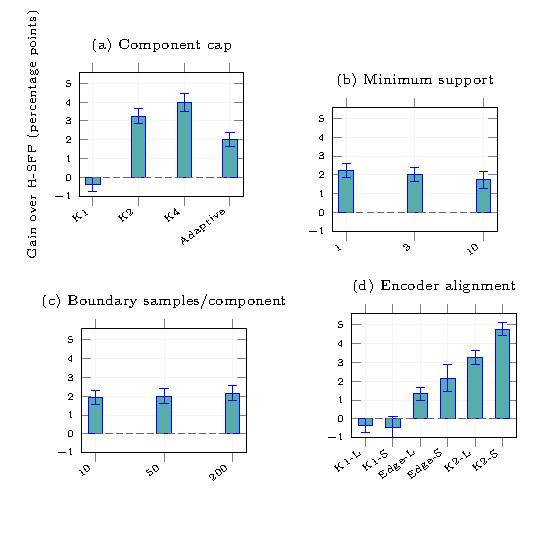
\includegraphics[width=\columnwidth]{figures/diagnostic_results.pdf}
\caption{Sensitivity and encoder-compatibility diagnostics after 200 rounds on CIFAR-100, Dir($\alpha=0.1$). Values are accuracy gains over the matched H-SFP mean of $5.49\%$. Error bars show $\sqrt{s_{\mathrm{method}}^2+s_{\mathrm{H\text{-}SFP}}^2}$ as descriptive dispersion, not paired-difference SDs or confidence intervals. Panels compare (a) component configurations, (b) minimum component support, (c) boundary Monte Carlo samples per component, and (d) local (L) and shared-snapshot (S) extraction.}
\label{fig:diagnostics}
\end{figure}

\subsection{Communication and Resource Costs}

\noindent\textbf{Communication breakdown.} \Cref{tab:resources} reports cumulative communication, runtime, and peak allocated memory under Dir($\alpha=0.1$). The analytical packet-body expression in \cref{eq:bytes} describes individual messages; the measured totals additionally include packet headers, repeated transmissions, and model synchronization.
Model synchronization contributes $4285.1\pm0.0$\,MiB to every listed configuration and dominates total traffic. K2 and K4 use $4724.7\pm2.4$\,MiB and $4776.8\pm3.7$\,MiB in total, compared with $4541.2\pm1.3$\,MiB for H-SFP, giving increases of approximately 4.0\% and 5.2\%.

The prototype-specific increases are substantially larger. Subtracting synchronization from the rounded H-SFP total gives approximately 256.1\,MiB of prototype traffic. K2 and K4 transmit 439.57 and 491.64\,MiB across the two boundaries, corresponding to increases of approximately 71.6\% and 92.0\%. Thus, the modest total-communication increments depend on the synchronization-dominated operating point. Both prototype traffic and total traffic are needed to assess the cost of retaining additional components.

\begin{table*}[t]
\caption{Communication and resource costs after 200 rounds on CIFAR-100, Dir($\alpha=0.1$): mean $\pm$ SD over three seeds. C--E and E--C denote client--edge and edge--cloud prototype traffic. Total communication includes $4285.1\pm0.0$\,MiB of model synchronization for every method. The boundary-specific prototype breakdown is unavailable for H-SFP. Measured packet sizes include headers, which are excluded from the body-size expression in \cref{eq:bytes}.}
\label{tab:resources}
\centering
\footnotesize
\setlength{\tabcolsep}{4pt}
\begin{tabular*}{\textwidth}{@{\extracolsep{\fill}}lccccc@{}}
\toprule
Method & C--E (MiB) & E--C (MiB) & Total (MiB) & Runtime (s) & Peak memory (MiB)\\
\midrule
H-SFP & n/a & n/a & $4541.2\pm1.3$ & $70398\pm1859$ & $2150\pm6$\\
MiSFP-K1 & $120.03\pm0.17$ & $142.06\pm1.42$ & $4547.2\pm1.4$ & $70579\pm1794$ & $2151\pm5$\\
MiSFP-Edge & $120.03\pm0.17$ & $235.65\pm0.33$ & $4640.8\pm0.5$ & $68828\pm169$ & $2150\pm5$\\
MiSFP-K2 & $150.90\pm0.75$ & $288.67\pm1.79$ & $4724.7\pm2.4$ & $68940\pm138$ & $2149\pm6$\\
MiSFP-K4 & $176.74\pm1.29$ & $314.90\pm2.72$ & $4776.8\pm3.7$ & $69208\pm295$ & $2151\pm5$\\
MiSFP-Adaptive & $127.92\pm0.15$ & $248.65\pm0.71$ & $4661.7\pm0.9$ & $70840\pm1656$ & $2151\pm5$\\
\bottomrule
\end{tabular*}
\end{table*}

\noindent\textbf{Packet-budget sensitivity.} Budget ratios are defined relative to the configured float32 K1 reference cap at each boundary. A float16 K2 configuration using the $1.0\times$ reference caps achieves $8.86\pm0.31\%$ accuracy with $4494.7\pm2.2$\,MiB total communication. Relative to matched H-SFP, this configuration gains 3.37 points while using approximately 1.0\% less total communication. Equal per-packet caps do not imply equal cumulative traffic because packet occupancy and retained component counts vary.
At $1.5\times$ and $2.0\times$ the reference cap, K2 reaches $8.48\pm0.24\%$ and $8.87\pm0.07\%$. Adaptive reaches $7.46\pm0.16\%$, $7.49\pm0.22\%$, and $7.32\pm0.22\%$ at $1.0\times$, $1.5\times$, and $2.0\times$, respectively. Across the tested configurations, larger caps are not associated with uniformly higher mean accuracy. The float16 matched setting jointly changes precision and component retention, so its result does not isolate either factor.

\noindent\textbf{Runtime and memory.} Mean runtimes range from 68828 to 70840 seconds, without a monotonic ordering by component count. Peak allocated GPU-memory means remain between 2149 and 2151\,MiB. These observations characterize the shared-GPU execution setting; they do not establish a runtime advantage, negligible incremental overhead, or per-client memory savings. The complexity analysis in \cref{sec:analysis} describes scaling, while isolated measurements of construction, merging, sampling, and boundary estimation are needed to quantify practical overhead.

\subsection{Representation Fidelity and Encoder Compatibility}

\noindent\textbf{Mixtures versus moment collapse.} \Cref{tab:fidelity} compares each K2 mixture with a single diagonal Gaussian derived from the same packet and matched to its unfloored diagonal moments. This controls the source packet while examining the effect of retaining multiple components.
Mixtures have lower mean SWD and MMD under both extraction regimes. Local-extraction MMD decreases from $0.1368\pm0.0151$ to $0.1221\pm0.0141$, while shared-snapshot MMD decreases from $0.0664\pm0.0016$ to $0.0530\pm0.0012$. In contrast, mixture NLL is higher in both regimes and varies substantially across seeds. Negative NLL values are valid for continuous densities.

These results support a metric-dependent interpretation: retaining components reduces the reported sample-based discrepancies but does not improve held-out likelihood. The comparison evaluates component retention within the diagonal-covariance interface; it does not establish superiority over richer covariance models. SWD and MMD also do not numerically evaluate the conditional loss bound in \cref{sec:analysis}.

\begin{table*}[t]
\caption{Representation fidelity and encoder compatibility on held-out real features after 200 rounds: mean $\pm$ SD over three seeds. Lower NLL, SWD, and MMD are better. The between-source ratio is computed from real features and is shared by both representations within each extraction regime.}
\label{tab:fidelity}
\centering
\footnotesize
\setlength{\tabcolsep}{4pt}
\begin{tabular*}{\textwidth}{@{\extracolsep{\fill}}llcccc@{}}
\toprule
Extraction & Representation & NLL (nat/dim) & SWD & MMD & Between-source ratio\\
\midrule
Local & Single Gaussian (collapsed K2 packet) & $-0.867\pm0.037$ & $0.053\pm0.004$ & $0.1368\pm0.0151$ & $0.474\pm0.049$\\
Local & MiSFP-K2 mixture & $-0.312\pm0.339$ & $0.051\pm0.005$ & $0.1221\pm0.0141$ & $0.474\pm0.049$\\
Shared snapshot & Single Gaussian (collapsed K2 packet) & $-0.970\pm0.050$ & $0.033\pm0.001$ & $0.0664\pm0.0016$ & $0.346\pm0.078$\\
Shared snapshot & MiSFP-K2 mixture & $-0.429\pm0.407$ & $0.031\pm0.001$ & $0.0530\pm0.0012$ & $0.346\pm0.078$\\
\bottomrule
\end{tabular*}
\end{table*}

\noindent\textbf{Shared encoder snapshot.} Local extraction uses each client's updated encoder, whereas shared-snapshot extraction uses a common encoder checkpoint. Fig.~\ref{fig:diagnostics}(d) compares these regimes for K1, Edge, and K2. The between-source dispersion ratio decreases from $0.474\pm0.049$ to $0.346\pm0.078$. This is consistent with encoder differences contributing to source separation, but dispersion alone cannot determine whether an individual component represents a semantic subpopulation.

With shared-snapshot extraction, K2 accuracy increases from $8.75\pm0.16\%$ to $10.26\pm0.05\%$. K1 changes little, reaching $5.04\pm0.47\%$ compared with $5.12\pm0.11\%$ under local extraction. K2 therefore retains a positive accuracy difference over K1 in both regimes. This supports the utility of retaining components under both extraction settings without identifying the semantic origin of the retained structure.

The intervention changes the encoder checkpoint as well as coordinate comparability, and a common client encoder does not guarantee alignment of independently trained edge-output mappings. It also raises total communication to $15060.3\pm2.5$\,MiB, approximately $3.19$ times the local-extraction K2 total of $4724.7\pm2.4$\,MiB. The shared-snapshot result is therefore interpreted as a sensitivity analysis with additional communication cost.